\documentclass[12pt, aspectratio=169]{beamer}

\usepackage{ctex}
\usepackage{amsmath, amssymb, amsfonts}
\usepackage{graphicx}
\usepackage{booktabs}
\usepackage{tikz}
\usepackage{multicol}
\usepackage{array}

% 主题设置
\usetheme{Madrid}
\usecolortheme{default}
% \usefonttheme{professionalfonts} % 保持数学字体美观

% 标题信息
\title{第三章：深度学习中的标准分布 - 概念解析与习题}
\subtitle{从离散分布到非参数方法}
% \institute{}
\author{《深度学习基础》课程小组}
\date{\today}

% 自定义命令
\newcommand{\vect}[1]{\mathbf{#1}}
\newcommand{\mat}[1]{\mathbf{#1}}
\newcommand{\R}{\mathbb{R}}
\newcommand{\E}{\mathbb{E}}
\newcommand{\N}{\mathcal{N}}
\newcommand{\Exp}{\text{Exp}}
\newcommand{\KL}{\mathrm{KL}}
\newcommand{\Tr}{\mathrm{Tr}}
\newcommand{\Hent}{\mathrm{H}}

\begin{document}

% 封面页
\begin{frame}
    \titlepage
\end{frame}

% 目录页
\begin{frame}{目录}
    \tableofcontents
\end{frame}


\section{深度学习中的标准分布的知识图谱}
\begin{frame}
    \frametitle{深度学习中的标准分布的知识图谱}
    \begin{center}
    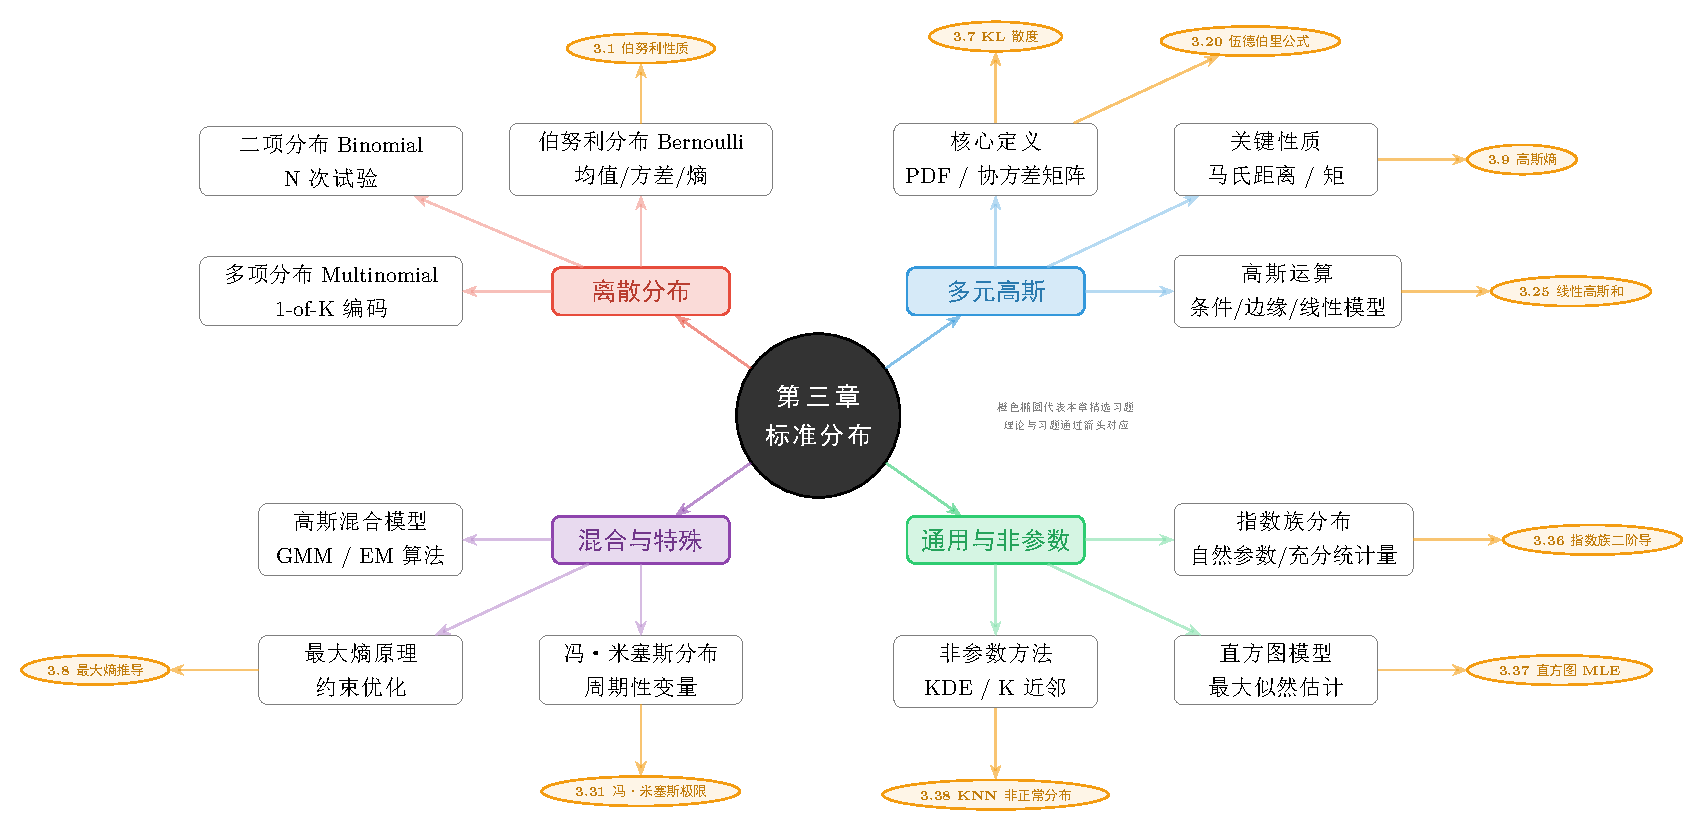
\includegraphics[width=0.95\textwidth]{ch03-graph.pdf}
    \end{center}
\end{frame}


\section{离散概率分布}

% 1. Bernoulli distribution
\begin{frame}{伯努利分布 (Bernoulli Distribution)}
    \begin{itemize}
        \item \textbf{定义}：描述单次二元试验（如抛硬币）结果的分布。
        \item \textbf{变量}：$x \in \{0, 1\}$，其中 $1$ 代表“成功”，$0$ 代表“失败”。
        \item \textbf{参数}：$\mu = p(x=1)$，即成功的概率，$0 \le \mu \le 1$。
        \item \textbf{概率质量函数 (PMF)}：
        $$ \text{Bern}(x|\mu) = \mu^x (1-\mu)^{1-x} $$
        \item \textbf{数字特征}：
        \begin{itemize}
            \item 均值：$\E[x] = \mu$
            \item 方差：$\text{Var}[x] = \mu(1-\mu)$
        \end{itemize}
        \item \textbf{应用}：二分类问题的输出层（如逻辑回归），生成式建模中的二值像素。
    \end{itemize}
\end{frame}

% 2. Binomial distribution
\begin{frame}{二项分布 (Binomial Distribution)}
    \begin{itemize}
        \item \textbf{定义}：描述 $N$ 次独立的伯努利试验中，“成功”次数 $m$ 的分布。
        \item \textbf{变量}：$m \in \{0, 1, \dots, N\}$。
        \item \textbf{参数}：$N$ (试验次数), $\mu$ (单次成功概率)。
        \item \textbf{概率质量函数}：
        $$ \text{Bin}(m|N, \mu) = \binom{N}{m} \mu^m (1-\mu)^{N-m} $$
        其中 $\binom{N}{m} = \frac{N!}{m!(N-m)!}$ 是组合数。
        \item \textbf{数字特征}：
        \begin{itemize}
            \item 均值：$\E[m] = N\mu$
            \item 方差：$\text{Var}[m] = N\mu(1-\mu)$
        \end{itemize}
        \item \textbf{联系}：当 $N=1$ 时，退化为伯努利分布。
    \end{itemize}
\end{frame}

% 3. Multinomial distribution
\begin{frame}{多项分布 (Multinomial Distribution)}
    \begin{itemize}
        \item \textbf{定义}：二项分布向多类别的推广。描述 $N$ 次独立试验中，$K$ 个互斥类别各自出现次数 $m_1, \dots, m_K$ 的联合分布。
        \item \textbf{变量}：$\vect{m} = (m_1, \dots, m_K)^T$，满足 $\sum m_k = N$。
        \item \textbf{参数}：$\boldsymbol{\mu} = (\mu_1, \dots, \mu_K)^T$，其中 $\sum \mu_k = 1$。
        \item \textbf{概率质量函数}：
        $$ \text{Mult}(\vect{m}|N, \boldsymbol{\mu}) = \frac{N!}{m_1! m_2! \cdots m_K!} \prod_{k=1}^K \mu_k^{m_k} $$
        \item \textbf{1-of-K 编码}：若只观察一次试验 ($N=1$)，则变量为向量 $\vect{x}$，其中仅有一个分量 $x_k=1$，其余为 0。此时 $p(\vect{x}|\boldsymbol{\mu}) = \prod_{k=1}^K \mu_k^{x_k}$。
        \item \textbf{应用}：多分类问题的标签分布，词袋模型 (Bag of Words)。
    \end{itemize}
\end{frame}

\section{多元高斯分布 (Multivariate Gaussian)}

% 4. Multivariate Gaussian
\begin{frame}{多元高斯分布 (Multivariate Gaussian Distribution)}
    \begin{itemize}
        \item \textbf{定义}：连续变量中最重要、最常用的分布，由均值向量和协方差矩阵完全确定。
        \item \textbf{变量}：$\vect{x} \in \R^D$。
        \item \textbf{参数}：
        \begin{itemize}
            \item 均值向量 $\boldsymbol{\mu} \in \R^D$。
            \item 协方差矩阵 $\boldsymbol{\Sigma} \in \R^{D \times D}$ (对称正定)。
        \end{itemize}
        \item \textbf{概率密度函数 (PDF)}：
        $$ \N(\vect{x}|\boldsymbol{\mu}, \boldsymbol{\Sigma}) = \frac{1}{(2\pi)^{D/2} |\boldsymbol{\Sigma}|^{1/2}} \exp\left( -\frac{1}{2} (\vect{x}-\boldsymbol{\mu})^T \boldsymbol{\Sigma}^{-1} (\vect{x}-\boldsymbol{\mu}) \right) $$
        \item \textbf{性质}：
        \begin{itemize}
            \item 等高线是椭圆（由 $\boldsymbol{\Sigma}$ 的特征向量决定方向）。
            \item 中心极限定理的基础。
        \end{itemize}
    \end{itemize}
\end{frame}

% 5. Mahalanobis distance
\begin{frame}{马氏距离 (Mahalanobis Distance)}
    \begin{itemize}
        \item \textbf{定义}：考虑了数据相关性（协方差）的距离度量，表示点 $\vect{x}$ 到分布中心 $\boldsymbol{\mu}$ 的“标准差”倍数。
        \item \textbf{公式}：
        $$ \Delta^2 = (\vect{x} - \boldsymbol{\mu})^T \boldsymbol{\Sigma}^{-1} (\vect{x} - \boldsymbol{\mu}) $$
        \item \textbf{几何意义}：
        \begin{itemize}
            \item 如果 $\boldsymbol{\Sigma} = \mat{I}$ (单位矩阵)，退化为欧几里得距离。
            \item 如果特征间存在相关性或量纲不同，马氏距离会自动进行“白化” (Whitening) 变换，消除相关性和尺度影响。
        \end{itemize}
        \item \textbf{在高斯分布中的作用}：高斯 PDF 中的指数部分正是 $-\frac{1}{2}\Delta^2$。常数马氏距离的轨迹构成了高斯分布的椭球等高面。
    \end{itemize}
\end{frame}

% 6. Moments of the Gaussian distribution
\begin{frame}{高斯分布的矩 (Moments of the Gaussian Distribution)}
    \begin{itemize}
        \item \textbf{一阶矩 (均值)}：
        $$ \E[\vect{x}] = \boldsymbol{\mu} $$
        \item \textbf{二阶中心矩 (协方差)}：
        $$ \E[(\vect{x}-\boldsymbol{\mu})(\vect{x}-\boldsymbol{\mu})^T] = \boldsymbol{\Sigma} $$
        \item \textbf{高阶矩}：
        \begin{itemize}
            \item 所有奇数阶中心矩为 0 (由于对称性)。
            \item 偶数阶矩可以通过 $\boldsymbol{\Sigma}$ 的组合表示 (Isserlis' theorem / Wick's probability theorem)。
            \item 例如：$\E[x_i x_j x_k x_l]$ 可以分解为协方差项的乘积之和。
        \end{itemize}
        \item \textbf{重要性}：高斯分布完全由其一阶和二阶矩决定，高阶矩不提供额外信息。这在许多近似推断方法（如卡尔曼滤波、变分推断）中非常关键。
    \end{itemize}
\end{frame}

% 7. Conditional distribution in a multivariate Gaussian
\begin{frame}{多元高斯的条件分布 (Conditional Distribution)}
    \begin{itemize}
        \item \textbf{设定}：将 $\vect{x}$ 划分为 $\vect{x}_a$ 和 $\vect{x}_b$。
        $$ \vect{x} = \begin{pmatrix} \vect{x}_a \\ \vect{x}_b \end{pmatrix}, \quad \boldsymbol{\mu} = \begin{pmatrix} \boldsymbol{\mu}_a \\ \boldsymbol{\mu}_b \end{pmatrix}, \quad \boldsymbol{\Sigma} = \begin{pmatrix} \boldsymbol{\Sigma}_{aa} & \boldsymbol{\Sigma}_{ab} \\ \boldsymbol{\Sigma}_{ba} & \boldsymbol{\Sigma}_{bb} \end{pmatrix} $$
        \item \textbf{性质}：给定 $\vect{x}_b$，$\vect{x}_a$ 的条件分布仍然是高斯分布 $p(\vect{x}_a|\vect{x}_b) = \N(\vect{x}_a | \boldsymbol{\mu}_{a|b}, \boldsymbol{\Sigma}_{a|b})$。
        \item \textbf{条件均值}：
        $$ \boldsymbol{\mu}_{a|b} = \boldsymbol{\mu}_a + \boldsymbol{\Sigma}_{ab}\boldsymbol{\Sigma}_{bb}^{-1}(\vect{x}_b - \boldsymbol{\mu}_b) $$
        (这是 $\vect{x}_b$ 的线性函数)
        \item \textbf{条件协方差}：
        $$ \boldsymbol{\Sigma}_{a|b} = \boldsymbol{\Sigma}_{aa} - \boldsymbol{\Sigma}_{ab}\boldsymbol{\Sigma}_{bb}^{-1}\boldsymbol{\Sigma}_{ba} $$
        (与 $\vect{x}_b$ 的具体值无关，仅取决于协方差结构)
        \item \textbf{应用}：高斯过程回归、卡尔曼滤波、贝叶斯网络推断。
    \end{itemize}
\end{frame}

% 8. Marginal distribution in a multivariate Gaussian
\begin{frame}{多元高斯的边缘分布 (Marginal Distribution)}
    \begin{itemize}
        \item \textbf{设定}：同上，将 $\vect{x}$ 划分为 $\vect{x}_a$ 和 $\vect{x}_b$。
        \item \textbf{性质}：对 $\vect{x}_b$ 积分（边缘化）后，$\vect{x}_a$ 的边缘分布仍然是高斯分布 $p(\vect{x}_a) = \N(\vect{x}_a | \boldsymbol{\mu}_a, \boldsymbol{\Sigma}_{aa})$。
        \item \textbf{结果}：
        \begin{itemize}
            \item 边缘均值：直接取对应部分的均值 $\boldsymbol{\mu}_a$。
            \item 边缘协方差：直接取对应部分的子矩阵 $\boldsymbol{\Sigma}_{aa}$。
        \end{itemize}
        \item \textbf{对比条件分布}：
        \begin{itemize}
            \item 边缘化非常简单（直接切分矩阵）。
            \item 条件分布需要矩阵求逆和舒尔补 (Schur Complement) 运算。
        \end{itemize}
        \item \textbf{意义}：高斯分布在边缘化操作下是封闭的，这使得在处理潜变量模型时非常方便。
    \end{itemize}
\end{frame}

% 9. Linear-Gaussian model
\begin{frame}{线性高斯模型 (Linear-Gaussian Model)}
    \begin{itemize}
        \item \textbf{定义}：涉及两个高斯分布的线性变换模型。
        \begin{itemize}
            \item 先验：$p(\vect{x}) = \N(\vect{x}|\boldsymbol{\mu}_x, \boldsymbol{\Lambda}^{-1})$
            \item 条件似然：$p(\vect{y}|\vect{x}) = \N(\vect{y}|\mat{A}\vect{x}+\vect{b}, \mat{L}^{-1})$
        \end{itemize}
        \item \textbf{结论 1 (边缘分布)}：$p(\vect{y})$ 是高斯分布。
        \item \textbf{结论 2 (后验分布)}：$p(\vect{x}|\vect{y})$ 也是高斯分布。
        \item \textbf{解析解}：
        \begin{itemize}
            \item 这种模型的边缘分布和后验分布的均值和协方差都有解析解（涉及矩阵求逆引理）。
        \end{itemize}
        \item \textbf{应用}：
        \begin{itemize}
            \item 因子分析 (Factor Analysis)。
            \item 线性动态系统 (Linear Dynamical Systems)。
            \item 卡尔曼滤波 (Kalman Filter) 的核心推导基础。
        \end{itemize}
    \end{itemize}
\end{frame}

% 10. Maximum likelihood estimate for mean and covariance
\begin{frame}{多元高斯的极大似然估计 (MLE for Mean \& Covariance)}
    \begin{itemize}
        \item \textbf{设定}：给定独立同分布数据集 $\mat{X} = \{\vect{x}_1, \dots, \vect{x}_N\}$。
        \item \textbf{均值的 MLE}：样本均值。
        $$ \boldsymbol{\mu}_{\text{ML}} = \frac{1}{N} \sum_{n=1}^N \vect{x}_n $$
        \item \textbf{协方差的 MLE}：样本协方差（有偏估计）。
        $$ \boldsymbol{\Sigma}_{\text{ML}} = \frac{1}{N} \sum_{n=1}^N (\vect{x}_n - \boldsymbol{\mu}_{\text{ML}})(\vect{x}_n - \boldsymbol{\mu}_{\text{ML}})^T $$
        \item \textbf{偏差问题}：
        $\boldsymbol{\Sigma}_{\text{ML}}$ 低估了真实的协方差。
        无偏估计量为：$\tilde{\boldsymbol{\Sigma}} = \frac{1}{N-1} \sum (\dots)$。
        \item \textbf{深度学习视角}：在批量归一化 (Batch Norm) 中，我们计算 mini-batch 的均值和方差，需注意训练时使用移动平均，而测试时使用全局统计量或修正后的无偏估计。
    \end{itemize}
\end{frame}

\section{混合模型与特殊分布}

% 11. Mixture of Gaussians
\begin{frame}{高斯混合模型 (Mixture of Gaussians, GMM)}
    \begin{itemize}
        \item \textbf{动机}：单个高斯分布是单峰的，无法拟合多峰复杂分布。
        \item \textbf{定义}：$K$ 个高斯分布的线性叠加。
        $$ p(\vect{x}) = \sum_{k=1}^K \pi_k \N(\vect{x}|\boldsymbol{\mu}_k, \boldsymbol{\Sigma}_k) $$
        \item \textbf{参数}：
        \begin{itemize}
            \item $\pi_k$：混合系数 (Mixing coefficients)，满足 $\sum \pi_k = 1, \pi_k \ge 0$。
            \item $\boldsymbol{\mu}_k, \boldsymbol{\Sigma}_k$：第 $k$ 个分量的均值和协方差。
        \end{itemize}
        \item \textbf{隐变量视角}：引入离散隐变量 $z$ 表示样本属于哪个分量，$p(z_k=1)=\pi_k$。
        \item \textbf{求解}：由于对数似然函数中包含求和的对数 $\ln \sum$，没有解析解。通常使用 \textbf{EM 算法} (Expectation-Maximization) 进行迭代优化。
        \item \textbf{应用}：聚类、密度估计、VAE 的先验近似。
    \end{itemize}
\end{frame}

% 12. Von Mises distribution
\begin{frame}{冯·米塞斯分布 (Von Mises Distribution)}
    \begin{itemize}
        \item \textbf{背景}：定义在圆环（周期性变量）上的分布，相当于线性空间中正态分布的循环版本。
        \item \textbf{变量}：角度 $\theta \in [0, 2\pi)$。
        \item \textbf{参数}：
        \begin{itemize}
            \item $\mu_0$：平均方向。
            \item $\kappa$：集中参数，类似精度的倒数。$\kappa=0$ 时为均匀分布，$\kappa$ 越大越集中。
        \end{itemize}
        \item \textbf{概率密度}：
        $\displaystyle p(\theta|\mu_0, \kappa) = \frac{1}{2\pi I_0(\kappa)} \exp(\kappa \cos(\theta - \mu_0)) $ \\ 
        其中 $I_0(\kappa)$ 是修正的零阶贝塞尔函数（归一化常数）。
        \item \textbf{应用}：
        \begin{itemize}
            \item 处理周期性数据（如时间、风向、机器人关节角度）。
            \item 在某些循环神经网络 (RNN) 或生成模型中用于建模角度输出。
        \end{itemize}
    \end{itemize}
\end{frame}

\section{通用理论与非参数方法}

% 13. The exponential family
\begin{frame}{指数族分布 (The Exponential Family)}
    \begin{itemize}
        \item \textbf{定义}：一大类概率分布的统称，其 PDF/PMF 可写成如下形式：
        $$ p(\vect{x}|\boldsymbol{\eta}) = h(\vect{x}) g(\boldsymbol{\eta}) \exp\left( \boldsymbol{\eta}^T \vect{u}(\vect{x}) \right) $$
        \item \textbf{组件}：
        \begin{itemize}
            \item $\boldsymbol{\eta}$：自然参数 (Natural parameters)。
            \item $\vect{u}(\vect{x})$：充分统计量 (Sufficient statistics)。
            \item $h(\vect{x})$：基底测度。
            \item $g(\boldsymbol{\eta})$：归一化系数。
        \end{itemize}
        \item \textbf{成员}：高斯、伯努利、二项、多项、泊松、Gamma、Beta 等。
        \item \textbf{重要性质}：
        \begin{itemize}
            \item 凸性：对数似然函数是关于 $\boldsymbol{\eta}$ 的凹函数，保证有唯一最大值。
            \item 充分统计量：数据的所有信息都压缩在 $\sum \vect{u}(\vect{x}_n)$ 中。
            \item 共轭先验：存在解析形式的共轭先验分布，便于贝叶斯推断。
        \end{itemize}
    \end{itemize}
\end{frame}

% 14. Nonparametric methods
\begin{frame}{非参数方法 (Nonparametric Methods)}
    \begin{itemize}
        \item \textbf{概念辨析}：
        \begin{itemize}
            \item \textbf{并非}“没有参数”，而是参数的数量不固定，通常随数据量 $N$ 的增长而增长。
            \item 不假设数据服从特定的参数化分布形式（如高斯）。
        \end{itemize}
        \item \textbf{特点}：
        \begin{itemize}
            \item \textbf{灵活性}：模型复杂度由数据决定，理论上可以逼近任意复杂的分布。
            \item \textbf{数据依赖}：预测新数据时通常需要保留全部或部分训练数据。
            \item \textbf{计算成本}：预测阶段计算量大（$O(N)$ 或更高），训练阶段快（通常只是存储数据）。
        \end{itemize}
        \item \textbf{典型代表}：
        \begin{itemize}
            \item 直方图 (Histograms)。
            \item 核密度估计 (KDE)。
            \item K近邻 (KNN)。
            \item 高斯过程 (Gaussian Processes)。
        \end{itemize}
    \end{itemize}
\end{frame}

% 15. Kernel density estimation
\begin{frame}{核密度估计 (Kernel Density Estimation, KDE)}
    \begin{itemize}
        \item \textbf{思想}：将每个数据点视为一个小的概率质量块（核函数），将所有核叠加得到整体密度。
        \item \textbf{公式}：
        $$ p(\vect{x}) = \frac{1}{N} \sum_{n=1}^N \frac{1}{h^D} k\left( \frac{\vect{x} - \vect{x}_n}{h} \right) $$
        \item \textbf{组件}：
        \begin{itemize}
            \item $k(\cdot)$：核函数（通常选高斯核），满足非负且积分为 1。
            \item $h$：带宽 (Bandwidth) 或平滑参数。
        \end{itemize}
        \item \textbf{带宽 $h$ 的作用}：
        \begin{itemize}
            \item $h$ 太小：过拟合，密度函数呈现尖锐的峰值（噪声大）。
            \item $h$ 太大：欠拟合，密度函数过于平滑，掩盖数据结构。
        \end{itemize}
        \item \textbf{联系}：可以看作是无限多个高斯分量的混合模型，每个分量中心在数据点上，权重相等。
    \end{itemize}
\end{frame}

% 16. Nearest-neighbour classifier
\begin{frame}{K近邻分类器 (Nearest-Neighbour Classifier)}
    \begin{itemize}
        \item \textbf{原理}：一种基于实例的非参数分类/回归方法。
        \item \textbf{算法}：
        \begin{enumerate}
            \item 对于新输入 $\vect{x}$，在训练集中找到距离最近的 $K$ 个点。
            \item \textbf{分类}：通过多数投票决定类别（$K=1$ 时即为最近邻）。
            \item \textbf{回归}：取 $K$ 个邻居目标值的平均值。
        \end{enumerate}
        \item \textbf{概率解释}：
        $$ p(\mathcal{C}_k|\vect{x}) \approx \frac{N_k}{K} $$
        其中 $N_k$ 是 $K$ 个邻居中属于类 $\mathcal{C}_k$ 的数量。
        \item \textbf{优缺点}：
        \begin{itemize}
            \item \textbf{优}：简单，无需训练，决策边界灵活。
            \item \textbf{缺}：预测慢（需计算所有距离），对高维数据失效（维数灾难），对噪声敏感（当 $K$ 较小时）。
        \end{itemize}
    \end{itemize}
\end{frame}

% 结束页
\begin{frame}{总结}
    \begin{itemize}
        \item \textbf{基础分布}：伯努利、二项、多项分布构成了离散变量建模的基石；多元高斯分布则是连续变量建模的核心。
        \item \textbf{高斯性质}：马氏距离、条件/边缘分布的封闭性、线性高斯模型的可解性，使得高斯分布在推断中占据统治地位。
        \item \textbf{复杂建模}：高斯混合模型 (GMM) 通过叠加突破单峰限制；冯·米塞斯分布处理周期性数据。
        \item \textbf{理论框架}：指数族统一了大多数常用分布的性质。
        \item \textbf{非参数视角}：当先验假设不足时，KDE 和 KNN 等方法利用数据本身驱动模型，虽计算昂贵但极具灵活性。
        \item 这些概率工具是理解变分自编码器 (VAE)、扩散模型 (Diffusion Models) 和高斯过程等现代深度学习算法的前提。
    \end{itemize}
\end{frame}

\section{标准分布的十个习题}

% % -----------------------------------------------------------
% % 习题 3.1: 伯努利分布性质
% % -----------------------------------------------------------
\begin{frame}{习题 3.1 ($\star$): 伯努利分布}
    \framesubtitle{伯努利分布的基本性质与熵}
    
    \textbf{问题描述：}
    验证伯努利分布 $\textrm{Bern}(x|\mu)=\mu^x(1-\mu)^{1-x}$ 满足以下基本性质：
    \begin{enumerate}
        \item \textbf{归一化}：$\displaystyle \sum_{x=0}^{1} p(x|\mu) = 1$
        \item \textbf{期望}：$\displaystyle \mathbb{E}[x] = \mu$
        \item \textbf{方差}：$\displaystyle \textrm{var}[x] = \mu(1-\mu)$
    \end{enumerate}
    
    % \vspace{1em}
    \textbf{进阶任务：}
    证明服从该分布的随机二元变量 $x$ 的熵 $\mathrm{H}[x]$ 为：
    \begin{equation*}
        \mathrm{H}[x] = -\mu \ln \mu - (1-\mu) \ln(1-\mu)
    \end{equation*}
    
    \textbf{提示：}
    熵的定义为 $\mathrm{H}[x] = -\sum p(x) \ln p(x)$。注意当 $x=0$ 和 $x=1$ 时的具体取值。
    
\end{frame}

% -----------------------------------------------------------
% 习题 3.7: 高斯分布的 KL 散度
% -----------------------------------------------------------
\begin{frame}{习题 3.7 ($\star\star\star$): 高斯分布的 KL 散度}
    \framesubtitle{两个多元高斯分布间的 KL 散度}
    
    \textbf{任务：}
    证明两个 $D$ 维高斯分布 $q(\vect{x}) = \mathcal{N}(\vect{x}|\boldsymbol{\mu}_q, \boldsymbol{\Sigma}_q)$ 和 $p(\vect{x}) = \mathcal{N}(\vect{x}|\boldsymbol{\mu}_p, \boldsymbol{\Sigma}_p)$ 之间的 Kullback-Leibler 散度为：
    \begin{equation*}
        \KL(q||p) = \frac{1}{2} \bigg\{ 
        \ln \frac{|\boldsymbol{\Sigma}_p|}{|\boldsymbol{\Sigma}_q|} - D 
        + \Tr\left(\boldsymbol{\Sigma}_p^{-1}\boldsymbol{\Sigma}_q\right) 
        + (\boldsymbol{\mu}_p - \boldsymbol{\mu}_q)^\mathrm{T} \boldsymbol{\Sigma}_p^{-1} (\boldsymbol{\mu}_p - \boldsymbol{\mu}_q) 
        \bigg\}
    \end{equation*}
    
    \begin{alertblock}{关键点}
    利用高斯分布的对数形式 $\ln \N(\vect{x}|\boldsymbol{\mu}, \boldsymbol{\Sigma})$ 展开计算期望。
    \end{alertblock}
\end{frame}

% -----------------------------------------------------------
% 习题 3.8: 最大熵原理
% -----------------------------------------------------------
\begin{frame}{习题 3.8 ($\star\star$): 最大熵原理}
    \framesubtitle{给定均值和协方差下的最大熵分布}
    
    \textbf{问题：}
    我们要证明：在所有具有指定均值 $\boldsymbol{\mu}$ 和协方差 $\boldsymbol{\Sigma}$ 的分布中，\textbf{高斯分布}具有最大的熵。即最大化熵泛函：
    \begin{equation*}
        \Hent[\vect{x}] = - \int p(\vect{x}) \ln p(\vect{x}) \,\mathrm{d}\vect{x}
    \end{equation*}
    
    \textbf{约束条件：}1. 归一化；2. 均值固定；3. 协方差固定：
    \begin{equation*}
        \int p(\vect{x}) \,\mathrm{d}\vect{x} = 1; \quad 
        \int p(\vect{x}) \vect{x} \,\mathrm{d}\vect{x} = \boldsymbol{\mu}; \quad 
        \int p(\vect{x}) (\vect{x}-\boldsymbol{\mu})(\vect{x}-\boldsymbol{\mu})^\mathrm{T} \,\mathrm{d}\vect{x} = \boldsymbol{\Sigma}. 
    \end{equation*}
    
    \textbf{任务：}
    使用\textbf{拉格朗日乘子法}对上述带约束问题进行变分最大化，证明最优解 $p(\vect{x})$ 即为高斯分布 $\N(\vect{x}|\boldsymbol{\mu},\boldsymbol{\Sigma})$。
\end{frame}

% -----------------------------------------------------------
% 习题 3.9: 高斯分布的熵
% -----------------------------------------------------------
\begin{frame}{习题 3.9 ($\star\star\star$): 高斯分布的熵}
    \framesubtitle{多元高斯分布熵的计算}
    
    \textbf{任务：}
    
    证明 $D$ 维多元高斯分布 $\N(\vect{x}|\boldsymbol{\mu}, \boldsymbol{\Sigma})$ 的熵由下式给出：
    
    \begin{equation*}
        \Hent[\vect{x}] = \frac{1}{2} \ln |\boldsymbol{\Sigma}| + \frac{D}{2} (1 + \ln(2\pi))
    \end{equation*}
    
    \vspace{1em}
    \begin{block}{推导思路}
        \begin{enumerate}
            \item 写出高斯分布的概率密度函数 $p(\vect{x})$。
            \item 代入熵的定义 $\Hent = -\E[\ln p(\vect{x})]$。
            \item 利用二次型 $\E[(\vect{x}-\boldsymbol{\mu})^\mathrm{T}\boldsymbol{\Sigma}^{-1}(\vect{x}-\boldsymbol{\mu})] = \Tr(\boldsymbol{\Sigma}^{-1}\boldsymbol{\Sigma}) = D$ 的性质简化计算。
        \end{enumerate}
    \end{block}
\end{frame}

% -----------------------------------------------------------
% 习题 3.20: 伍德伯里矩阵求逆公式
% -----------------------------------------------------------
\begin{frame}{习题 3.20 ($\star\star$): 伍德伯里矩阵求逆公式}
    \framesubtitle{验证伍德伯里恒等式 (Woodbury Identity)}
    
    \textbf{问题描述：}
    线性代数中著名的\textbf{伍德伯里矩阵求逆公式}形式如下：
    \begin{equation*}
        (\mat{A} + \mat{B}\mat{C}\mat{D})^{-1} = \mat{A}^{-1} - \mat{A}^{-1}\mat{B}(\mat{C}^{-1} + \mat{D}\mat{A}^{-1}\mat{B})^{-1}\mat{D}\mat{A}^{-1}
    \end{equation*}
    
    \vspace{0.5em}
    \textbf{任务：}
    通过将等式\textbf{右边}乘以 $(\mat{A} + \mat{B}\mat{C}\mat{D})$，证明结果为单位矩阵 $\mat{I}$，从而验证该公式的正确性。
    
    \vspace{0.5em}
    \begin{alertblock}{应用背景}
    该公式在机器学习中常用于高效更新协方差矩阵的逆（例如在卡尔曼滤波或高斯过程回归中），特别是当 $\mat{C}$ 的维度远小于 $\mat{A}$ 时。
    \end{alertblock}
\end{frame}

% -----------------------------------------------------------
% 习题 3.25: 独立高斯变量的和
% -----------------------------------------------------------
% \begin{frame}{习题 3.25 ($\star\star$): 独立高斯变量的和}
%     \framesubtitle{两个高斯分布之和的边缘分布}
    
%     \textbf{设定：}
%     $\mathbf{x} \sim \N(\boldsymbol{\mu}_{\mathbf{x}}, \boldsymbol{\Sigma}_{\mathbf{x}})$, \quad 
%     $\mathbf{z} \sim \N(\boldsymbol{\mu}_{\mathbf{z}}, \boldsymbol{\Sigma}_{\mathbf{z}})$, \quad 
%     $\mathbf{y} = \mathbf{x} + \mathbf{z}$
    
%     \textbf{任务：}
%     通过构建一个线性 - 高斯模型（考虑联合分布 $p(\mathbf{x}, \mathbf{y}) = p(\mathbf{x})p(\mathbf{y}|\mathbf{x})$
    
%     并利用线性高斯系统的通用性质：
%     \begin{align*}
%     \displaystyle \mathbb{E}[\mathbf{y}] &= \mathbf{A}\boldsymbol{\mu} + \mathbf{b} \\
%     \displaystyle \textrm{cov}[\mathbf{y}] &= \mathbf{L}^{-1} + \mathbf{A}\boldsymbol{\Lambda}^{-1}\mathbf{A}^\mathrm{T}
%     \end{align*}
    
%     证明 $\mathbf{y}$ 的边缘分布为：
%     \begin{equation*}
%         p(\mathbf{y}) = \N(\mathbf{y} | \boldsymbol{\mu}_{\mathbf{x}} + \boldsymbol{\mu}_{\mathbf{z}}, \; \boldsymbol{\Sigma}_{\mathbf{x}} + \boldsymbol{\Sigma}_{\mathbf{z}})
%     \end{equation*}
    
%     \begin{block}{结论}
%         独立高斯变量之和仍为高斯分布，其均值为均值之和，协方差为协方差之和。
%     \end{block}
% \end{frame}

% -----------------------------------------------------------
% 习题 3.25: 独立高斯变量的和
% -----------------------------------------------------------
\begin{frame}[allowframebreaks]{习题 3.25 ($\star\star$): 独立高斯变量的和}
    \framesubtitle{利用线性 - 高斯模型推导和的分布}
    
    \textbf{问题设定：}
    \begin{itemize}
        \item 随机向量 $\mathbf{x}$ 和 $\mathbf{z}$ \textbf{相互独立}。
        \item 分布分别为：$\mathbf{x} \sim \mathcal{N}(\boldsymbol{\mu}_{\mathbf{x}}, \boldsymbol{\Sigma}_{\mathbf{x}})$，$\mathbf{z} \sim \mathcal{N}(\boldsymbol{\mu}_{\mathbf{z}}, \boldsymbol{\Sigma}_{\mathbf{z}})$。
        \item 定义新变量：$\mathbf{y} = \mathbf{x} + \mathbf{z}$。
    \end{itemize}

    \vspace{0.5em}
    \textbf{任务：}
    不直接使用卷积公式，而是通过构建\textbf{线性 - 高斯模型}来推导 $p(\mathbf{y})$。
    
    \begin{enumerate}
        \item \textbf{构建条件分布}：将 $\mathbf{y}$ 视为给定 $\mathbf{x}$ 的线性变换加噪声。
        写出 $p(\mathbf{y}|\mathbf{x})$ 的形式，并识别出线性高斯模型的标准参数：
        $$ \mathbf{y} = \mathbf{A}\mathbf{x} + \mathbf{b} + \boldsymbol{\epsilon}, \quad \boldsymbol{\epsilon} \sim \mathcal{N}(\mathbf{0}, \boldsymbol{\Sigma}_{\boldsymbol{\epsilon}}) $$
        \item \textbf{应用通用性质}：利用线性高斯系统的边缘分布性质：
        \begin{align*}
            \mathbb{E}[\mathbf{y}] &= \mathbf{A}\boldsymbol{\mu}_{\mathbf{x}} + \mathbf{b} \\
            \textrm{cov}[\mathbf{y}] &= \boldsymbol{\Sigma}_{\boldsymbol{\epsilon}} + \mathbf{A}\boldsymbol{\Sigma}_{\mathbf{x}}\mathbf{A}^\mathrm{T}
        \end{align*}
        \item \textbf{得出结论}：证明 $\mathbf{y}$ 的边缘分布为：
        \begin{equation*}
            p(\mathbf{y}) = \mathcal{N}(\mathbf{y} \mid \boldsymbol{\mu}_{\mathbf{x}} + \boldsymbol{\mu}_{\mathbf{z}}, \; \boldsymbol{\Sigma}_{\mathbf{x}} + \boldsymbol{\Sigma}_{\mathbf{z}})
        \end{equation*}
    \end{enumerate}

    % \vspace{0.5em}
    \begin{alertblock}{关键提示}
        在此模型中，$\mathbf{z}$ 充当了加法噪声的角色。请确定 $\mathbf{A}$, $\mathbf{b}$ 和噪声协方差 $\boldsymbol{\Sigma}_{\boldsymbol{\epsilon}}$ 分别对应题目中的哪些量。
    \end{alertblock}
\end{frame}

% -----------------------------------------------------------
% 习题 3.31: 冯·米塞斯分布的高斯极限
% -----------------------------------------------------------
\begin{frame}{习题 3.31 ($\star\star$): 冯·米塞斯分布的高斯极限}
    \framesubtitle{冯·米塞斯分布在大浓度参数下的近似}
    
    \textbf{背景：}
    冯·米塞斯分布 (Von Mises distribution) 定义为：
    \begin{equation*}
        p(\theta|\theta_0,m) = \frac{1}{2\pi I_0(m)}\exp\{m\cos(\theta-\theta_0)\}
    \end{equation*}
    当浓度参数 $m$ 很大时，分布集中在众数 $\theta_0$ 附近。
    
    \vspace{1em}
    \textbf{任务：}
    1. 定义变换变量 $\xi = m^{1/2}(\theta - \theta_0)$。\\
    2. 对余弦项进行泰勒展开：$\cos \alpha \approx 1 - \frac{\alpha^2}{2}$。\\
    3. 证明当 $m \to \infty$ 时，该分布趋向于一个\textbf{高斯分布}。
    
    \vspace{1em}
    \footnotesize{提示：注意雅可比行列式的变化以及归一化常数 $I_0(m)$ 在大 $m$ 时的渐近行为。}
\end{frame}

% -----------------------------------------------------------
% 习题 3.36: 指数族的二阶性质
% -----------------------------------------------------------
\begin{frame}{习题 3.36 ($\star$): 指数族的二阶性质}
    \framesubtitle{指数族分布中 $\ln g(\mat{\eta})$ 的二阶导数}
    
    \textbf{已知结果：}
    对于指数族分布，$\ln g(\mat{\eta})$ 的一阶梯度与充分统计量的期望有关：
    \begin{equation*}
        -\nabla\ln g(\mat{\eta})=\E[\mathbf{u}(\vect{x})]
    \end{equation*}
    
    \textbf{任务：}
    从归一化条件出发：
    % \begin{equation*}
    $\displaystyle g(\mat{\eta})\int h(\vect{x})\exp\{\mat{\eta}^{\mathrm{T}}\mathbf{u}(\vect{x})\}\mathrm{d}\vect{x} = 1
    $
    % \end{equation*}

    对其取关于 $\mat{\eta}$ 的\textbf{二阶导数}，证明：
    % \begin{equation*}
    $\displaystyle
        -\nabla\nabla \ln g(\mat{\eta}) = \underbrace{\E[\mathbf{u}\mathbf{u}^\mathrm{T}] - \E[\mathbf{u}]\E[\mathbf{u}]^\mathrm{T}}_{\text{cov}[\mathbf{u}(\vect{x})]}
    $
    % \end{equation*}
    
    \begin{alertblock}{意义}
        这表明 $\ln g(\mat{\eta})$ 的负海森矩阵 (Hessian) 等于充分统计量的协方差矩阵，且协方差矩阵必须是半正定的，这意味着 $\ln g(\mat{\eta})$ 是凸函数。
    \end{alertblock}
\end{frame}

% -----------------------------------------------------------
% 习题 3.37: 直方图密度模型的 MLE
% -----------------------------------------------------------
\begin{frame}{习题 3.37 ($\star\star$): 直方图密度模型的 MLE}
    \framesubtitle{直方图模型的最大似然估计}
    
    \textbf{模型设定：}
    \begin{itemize}
        \item 空间被划分为固定区域 $i$。区域 $i$ 的体积为 $\Delta_i$。密度在区域 $i$ 内为常数 $h_i$。
        \item 观测数据：共 $N$ 个点，其中 $n_i$ 个落在区域 $i$。
    \end{itemize}
    
    \vspace{0.5em}
    \textbf{任务：}
    
    1. 写出该模型的对数似然函数。\\
    2. 使用\textbf{拉格朗日乘子法}强制执行归一化约束 $\sum_i h_i \Delta_i = 1$。\\
    3. 推导出 $\{h_i\}$ 的最大似然估计量表达式。
    
    \vspace{0.5em}
    \begin{block}{预期结果}
        估计值应与落入该区域的频率成正比，与区域体积成反比。
    \end{block}
\end{frame}

% -----------------------------------------------------------
% 习题 3.38: K 近邻模型的非正常性
% -----------------------------------------------------------
\begin{frame}{习题 3.38 ($\star$): K 近邻模型的非正常性}
    \framesubtitle{K 近邻密度模型的积分发散性}
    
    \textbf{问题描述：}
    $K$ 近邻 (K-Nearest Neighbors, KNN) 密度估计模型定义为：
    \begin{equation*}
        p(\vect{x}) = \frac{K}{N V(\vect{x})}
    \end{equation*}
    其中 $V(\vect{x})$ 是以 $\vect{x}$ 为中心、恰好包含 $K$ 个训练数据点的超球体体积。
    
    \textbf{任务：}
    证明该模型定义了一个\textbf{非正常分布} (Improper Distribution)，即其在整个空间上的积分是发散的：
    \begin{equation*}
        \int p(\vect{x}) \,\mathrm{d}\vect{x} = \infty
    \end{equation*}
    
    \begin{alertblock}{直观理解}
        考虑远离所有数据点的区域，$V(\vect{x})$ 会变得非常大但增长缓慢，导致尾部衰减不足以使积分收敛。
    \end{alertblock}
\end{frame}

\end{document}
